\documentclass[11pt]{article}
\usepackage{amsmath,amsthm,amssymb,fullpage,graphicx,hyperref,listings}
\usepackage{listings,color,setspace}
\author{Andy Reagan}
\title{Math 337 Homework 09}

     \def\NN{\mathbb{N} }
     \def\ZZ{\mathbb{Z} }
     \def\QQ{\mathbb{Q} }
     \def\RR{\mathbb{R} }
     \def\CC{\mathbb{C} }
     \def\f{\frac }
     \def\b{\begin }
     \def\e{\end }
     \def\Log{\text{Log} \,}
     \def\Re{\text{Re} \, }

\lstset{language=MATLAB,
basicstyle=\ttfamily\scriptsize\singlespacing,
keywordstyle=\color{black},
stringstyle=\color{black},
commentstyle=\color{black},
morecomment=[l][\color{black}]{\#},
frame=L,
xleftmargin=\parindent,
%%numbers=left,                   %% where to put the line-numbers
%%numberstyle=\scriptsize,      %% the size of the fonts that are used for the line-numbers
%%stepnumber=1,                   %% the step between two line-numbers. If it is 1 each line will be numbered
numbersep=5pt,
breaklines=true,        %% sets automatic line breaking
breakatwhitespace=false,    %% sets if automatic breaks should only happen at whitespace
escapeinside={\%*}{*)} 
}


     \newcommand{\pdiff}[2]{\frac{\partial #1}{\partial #2}}
     \newcommand{\partialdiff}[2]{\frac{\partial #1}{\partial #2}}
     \newcommand{\pdiffsq}[2]{\frac{\partial^2 #1}{{\partial #2}^2}}
     \newcommand{\pdiffcu}[2]{\frac{\partial^3 #1}{{\partial #2}^3}}
     \newcommand{\pdiffhi}[3]{\frac{\partial^#3 #1}{{\partial #2}^#3}}
     \newcommand{\diff}[2]{\frac{{\rm d}#1}{{\rm d}#2}}
     \newcommand{\diffsq}[2]{\frac{{\rm d}^{2}#1}{{\rm d} {#2}^2}}
     \newcommand{\diffhi}[3]{\frac{{\rm d}^#3 #1}{{\rm d} {#2}^#3}}
     \newcommand{\tdiff}[2]{\mbox{d} #1/\mbox{d} #2}
     \newcommand{\tdiffsq}[2]{\mbox{d}^{2} #1/\mbox{d} {#2}^2}
     \newcommand{\tpdiff}[2]{\partial #1/\partial #2}
     \newcommand{\tpdiffsq}[2]{\partial^2 #1/\partial {#2}^2}
     \newcommand{\bvec}[1]{\vec{ {\bf #1 } }}
     \newcommand{\oh}[1]{O(h^{{#1}})}

\begin{document}
\maketitle

\begin{enumerate}

\item Solve the BVP
\[ y'' - \f{2y}{(1+x)^2} = -\f{4}{(1+x)^2}, ~~~~~y(0)=0,~~~y(1) = 1\]
using the collocation method with $\phi _j = \sin (j\pi x)$ for $j = 1,\ldots,M$ and $M=10$.
Use the equidistant collocation points $x_k = x_0 + k\cdot h$.
Compare you finite-element solution with the exact solution $y_{\text{exact}} = 2x/(1+x)$ by plotting them together, and also by plotting, in a separate figure, the error for $x\in [0,1]$.

\bigskip
\textbf{Solution:} Using the hint, we make the change of variables $z(x) = y(x)-x$, and therefore the new problem has boundary conditions $z(0) = y(0) - 0 = 0$ and $z(1) = y(1) - 1 = 0$.
Noting that $y'' = z''$ and the definition $z = y-x$ we rewrite the BVP as
\[ z'' - \f{2z}{(1+x)^2} = -\f{4}{(1+x)^2} + \f{2x}{(1+x)^2}, ~~~~~z(0)=0,~~~z(1) = 0.\]

The solution is obtained by the following code, and I include plots of the numerical solution and exact solution (Figure 1), the error of that solution (Figure 2) and the scaling of error with $(1/M)$ (Figure 3).

\lstinputlisting[language=Matlab]{andy_hw09_prb01.m}

\begin{figure}[h!]
  \centering
    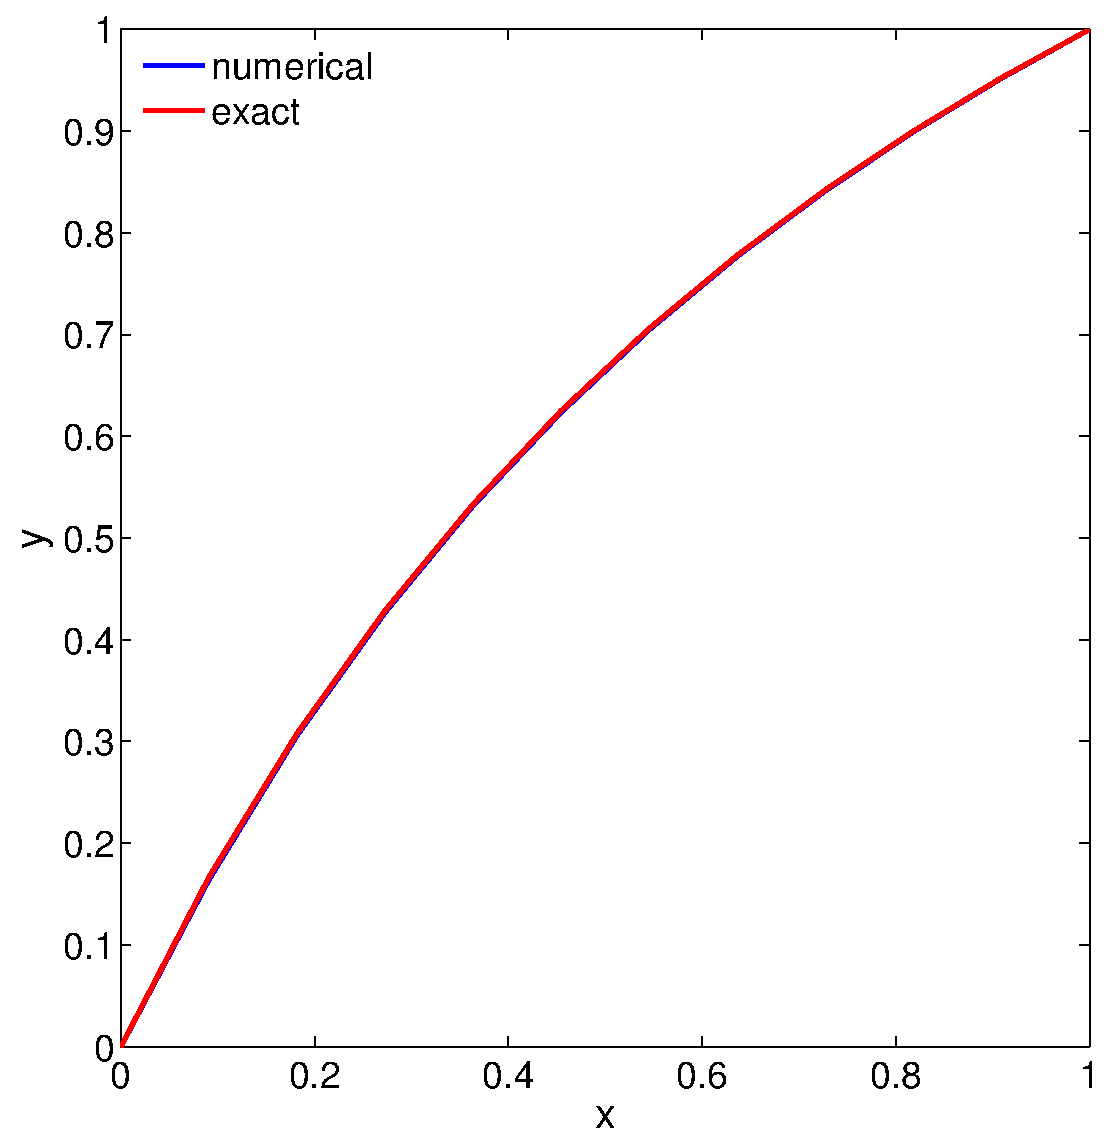
\includegraphics[width=0.45\textwidth]{andy_hw09_prb01_01_m10.pdf}
  \caption{Exact and numerical solutions of the BVP using the collocation method with $M=10$.}
\end{figure}

\begin{figure}[h!]
  \centering
    \includegraphics[width=0.45\textwidth]{andy_hw09_prb01_01_m10_error.pdf}
  \caption{Error of the solution to the BVP using the collocation method with $M=10$.}
\end{figure}

\begin{figure}[h!]
  \centering
    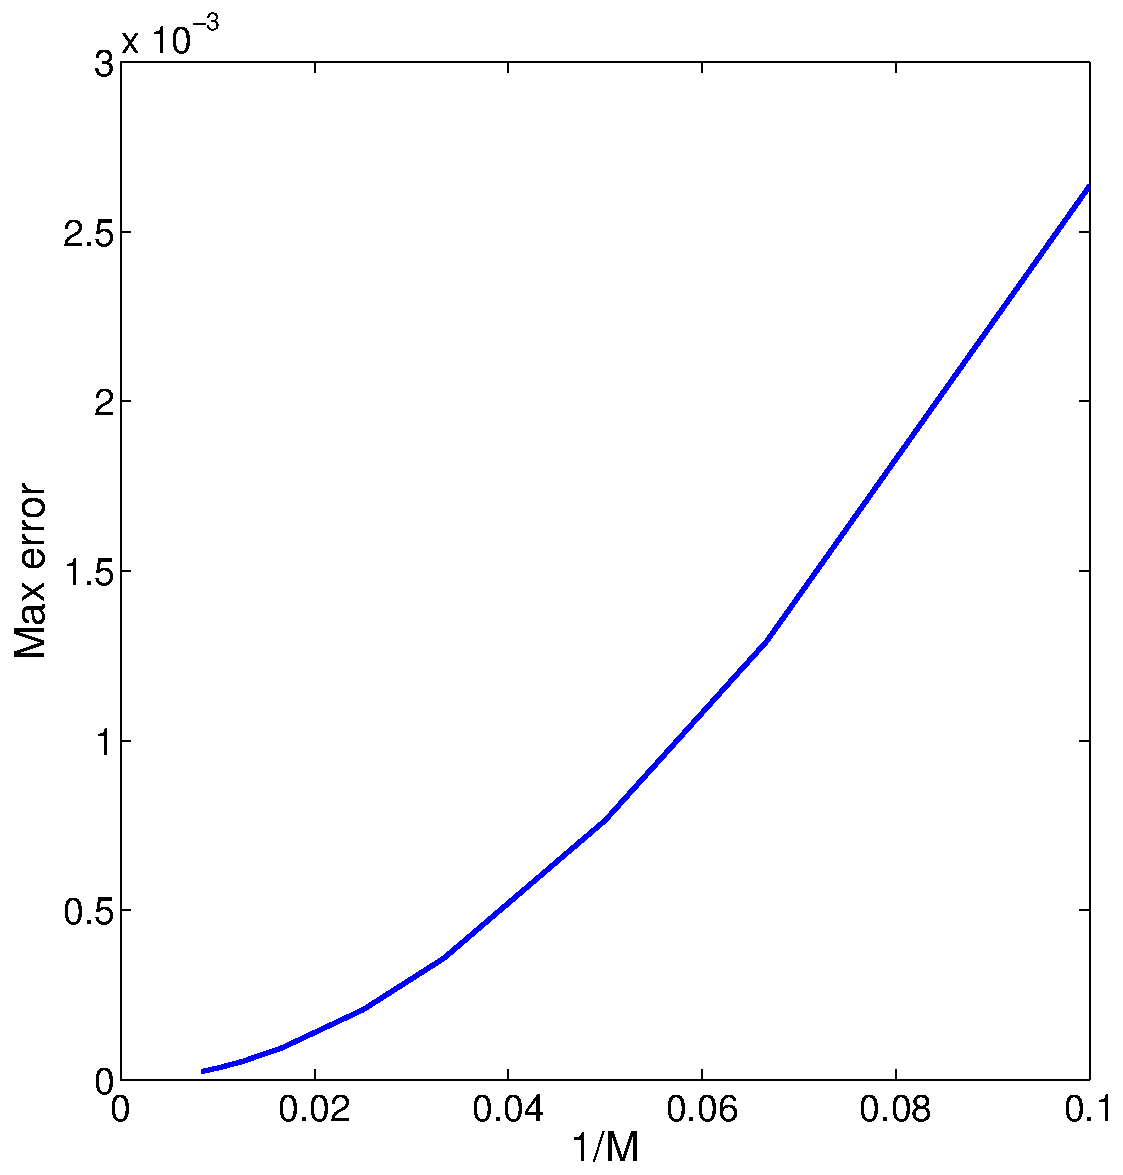
\includegraphics[width=0.45\textwidth]{andy_hw09_prb01_02.pdf}
  \caption{Scaling of the maximum error the collocation solution with $(1/M)$. We observe that error scales super-linearly (perhaps quadratically) with $1/M$, indicating that the error decrease scales sub-linearly with the decrease in $h$ (where by $h$ I mean the point spacing, which makes sense here, where the points are evenly spaced).}
\end{figure}

\item Obtain Eqs. (9.20) and (9.22) of the notes.

\bigskip
\textbf{Solution:} First we have that
\begin{equation*} \phi _j ' = \left\{ \begin{array}{cc} \f{1}{h} & x_{j-1} < x < x_j \\ \f{-1}{h} & x_j < x < x_{j+1} \\ 0~~~ & \text{otherwise}\end{array} \right. \end{equation*}
For $| k-j | > 1$ it is clear from the above function that the $\phi _k'(x) \phi _j'(x) = 0$. Therefore I consider the remaining three cases: $|k-j| = 1$ and $k=j$.

First, for $k=j$ we have that
\begin{equation*} \phi _j '(x) \phi_j '(x) = \left\{ \begin{array}{cc} \f{1}{h^2} & x_{j-1} < x < x_j \\ \f{1}{h^2} & x_j < x < x_{j+1} \\ 0~~~ & \text{otherwise}\end{array} \right. \end{equation*}
We write this more concisely as
\begin{equation*} \phi _j '(x) \phi_j '(x) = \left\{ \begin{array}{cc} \f{1}{h^2} & x_{j-1} < x < x_{j+1}, x\ne x_j \\ 0~~~ & \text{otherwise}\end{array} \right. \end{equation*}
The integral of this function is $x/h^2$, we don't worry about the single point $x_j$, and so we take the integral over the nonzero part of this function (the rest is 0) to obtain 
\begin{equation} \int _{x_{j-1}} ^{x_{j+1}} h^{-2}dx = \left. h^{-2}x \right |_{x_j-h}^{x_j+h} = \f{2}{h} .\end{equation}

Now consider $k = j-1$, and we have
\begin{equation*} \phi _{j-1} '(x) \phi_j '(x) = \left\{ \begin{array}{cc} \f{1}{h} & x_{j-2} < x < x_{j-1} \\ \f{-1}{h^2} & x_{j-1} < x < x_{j} \\ \f{1}{h} & x_{j} < x < x_{j+1} \\0~~~ & \text{otherwise}\end{array} \right. \end{equation*}
Considering the integral of all three pieces, we have
\begin{align*} \int _{x_{j-2}} ^{x_{j+1}} \phi _{j-1} '(x) \phi_j '(x) dx &= \int _{x_{j-2}} ^{x_{j-1}} \f{1}{h} dx + \int _{x_{j-1}} ^{x_{j}} \f{-1}{h^2} dx + \int _{x_{j}} ^{x_{j+1}} \f{-1}{h} dx \\
&= \left. \f{x}{h} \right | _{x_{j}-2h} ^{x_{j}-h} - \left. \f{x}{h^2} \right| _{x_{j}-h} ^{x_{j}} - \left. \f{x}{h} \right | _{x_{j}} ^{x_{j}+h} \\
&= 1 +\f{1}{h} - 1 = \f{1}{h} \end{align*}

The above applies to case $k=j+1$ by replacing all of the subscripts $j-2$ to $j+2$, $j+1$ to $j-1$ and $j-1$ to $j+1$ (or simply setting $h \to -h$ in the replacement).

Therefore we have Eq 9.20, as desired.

To compute the integral in Eq 9.22, first we (again) note that for $|k-j| >1 $ that $\phi_j(x) \phi _k(x) = 0$ for all $x$.
Again we consider the three remaining cases (and will argue that WLOG we only need show $k=j-1$ without $k=j+1$).

For $k=j$ we have
\begin{equation*} \phi _j (x) \phi_j (x) = \left\{ \begin{array}{cc} \left (1-\f{\left | \Delta x_j \right | }{h}\right ) ^2 & x_{j-1} < x < x_{j+1} \\ 0~~~ & \text{otherwise}\end{array} \right. \end{equation*}
Therefore we take the integral only on the nonzero part (the rest is 0) to obtain (changing variables $z = x-x_j$)
\begin{align*} \int _{x_{j-1}} ^{x_{j+1}} \phi _j (x) \phi_j (x) dx &= \int _{x_{j-1}} ^{x_{j+1}} \left (1-\f{\left | \Delta x_j \right | }{h}\right ) ^2 dx\\ 
&= \int _{x_j-h} ^{x_{j}+h} \left (1-\f{\left | x-x_j \right | }{h}\right ) ^2 dx\\ 
&= \int _{-h} ^{h} \left ( 1-\f{2\left | z \right | }{h} + \f{z^2}{h^2} \right )dz \\ 
&= \int _{0} ^{h} \left ( 1-\f{2z}{h} + \f{z^2}{h^2} \right )dz +\int _{-h} ^{0} \left ( 1-\f{2|z|}{h} + \f{z^2}{h^2} \right )dz \\ 
&= 2\int _{0} ^{h} \left ( 1-\f{2z}{h} + \f{z^2}{h^2} \right )dz \\
&= 2\left .\left ( z-\f{z^2}{h} + \f{z^3}{3h^2} \right )\right | _{0} ^h \\
&= 2\left ( h-\f{h^2}{h} + \f{h^3}{3h^2} \right ) = 2\left ( h-h+ \f{h}{3} \right ) = \f{2}{3} h\end{align*}

For $k=j-1$ we have the following integral:
\begin{align*} \int _{x_{j-2}} ^{x_{j+1}} \phi _{j-1} (x) \phi_j (x) dx &= \int _{x_{j-2}} ^{x_{j-1}} \left ( 1-\f{|x-x_{j-1}|}{h} \right ) ( 0 )dx + \int _{x_{j-1}} ^{x_{j}} \left ( 1- \f{|x-x_{j-1}|}{h}\right ) \left (  1- \f{|x-x_{j}|}{h}\right ) dx\\ &~~~~  + \int _{x_{j}} ^{x_{j+1}} \left ( 1-\f{|x-x_{j}|}{h} \right ) (0) dx \end{align*}
%% I solve these three integrals one by one.
%% The first integral, transforming $z = x-x_{j-1}$ becomes
%% \begin{align*} \int _{x_{j-2}} ^{x_{j-1}} 1-\f{|x-x_{j-1}|}{h} dx & = \int _{-h} ^{0} 1-\f{|z|}{h} dz\end{align*}

%% The last integral, transforming $z = x-x_{j}$ becomes
%% \begin{align*} \int _{x_{j}} ^{x_{j+1}} 1-\f{|x-x_{j}|}{h} dx & = \int _{0} ^{h} 1-\f{|z|}{h} dz\end{align*}

%% The first and last integrals are equal, and so we have
%% \begin{align*} 2 \int _{0} ^{h} 1-\f{z}{h} dz & = 2\left. \left ( z-\f{z^2}{2h}\right) \right | _0 ^h = h \end{align*}

The first and last integral are zero, so we are only concerned with the middle one.
The middle integral, transforming $z = x-x_{j-1}$ becomes
\begin{align*} \int _{x_{j-1}} ^{x_{j}} \left ( 1- \f{|x-x_{j-1}|}{h}\right ) \left (  1- \f{|x-x_{j}|}{h}\right ) dx &=  \int _{0} ^{h} \left ( 1- \f{|z|}{h}\right ) \left (  1- \f{|z-h|}{h}\right ) dz \\
&=  \int _{0} ^{h} \left ( 1- \f{z}{h}\right ) \left (  1+ \f{z-h}{h}\right ) dz \\
&=  \int _{0} ^{h}\left ( 1 + \f{z-h}{h} - \f{z}{h} - \f{z}{h}\f{z-h}{h}\right ) dz \\
&=  -\int _{0} ^{h} \left ( \f{z^2}{h^2}-\f{z}{h}\right ) dz \\
&=  \left. \f{z^2}{2h}-\f{z^3}{3h^2} \right | _{0} ^{h} = \f{h}{6} \end{align*}


\item Solve the BVP in Problem 1 by the Galerkin method with the hat functions and $M=10$.
Compare your result with the exact solution.
As in Problem 1, investigate how the error of the Galerkin method scales with $(1/M)$.

\bigskip
\textbf{Solution:} The solution is obtained by the following code, and I include plots of the numerical solution and exact solution (Figure 4), the error (Figure 5) and the scaling of error with $(1/M)$ (Figure 6).

I verified that my matrix is symmetric, and I can't find why my error is not as small as the figure you provide.
I tried using MATLAB's ``quad'' to do the integration of the integrals numerically, and this did not help.
Note that although there is a loop over $M$, the code only runs for $M=10$, on which I did all of my troubleshooting.

\lstinputlisting[language=Matlab]{andy_hw09_prb03.m}

\begin{figure}[h!]
  \centering
    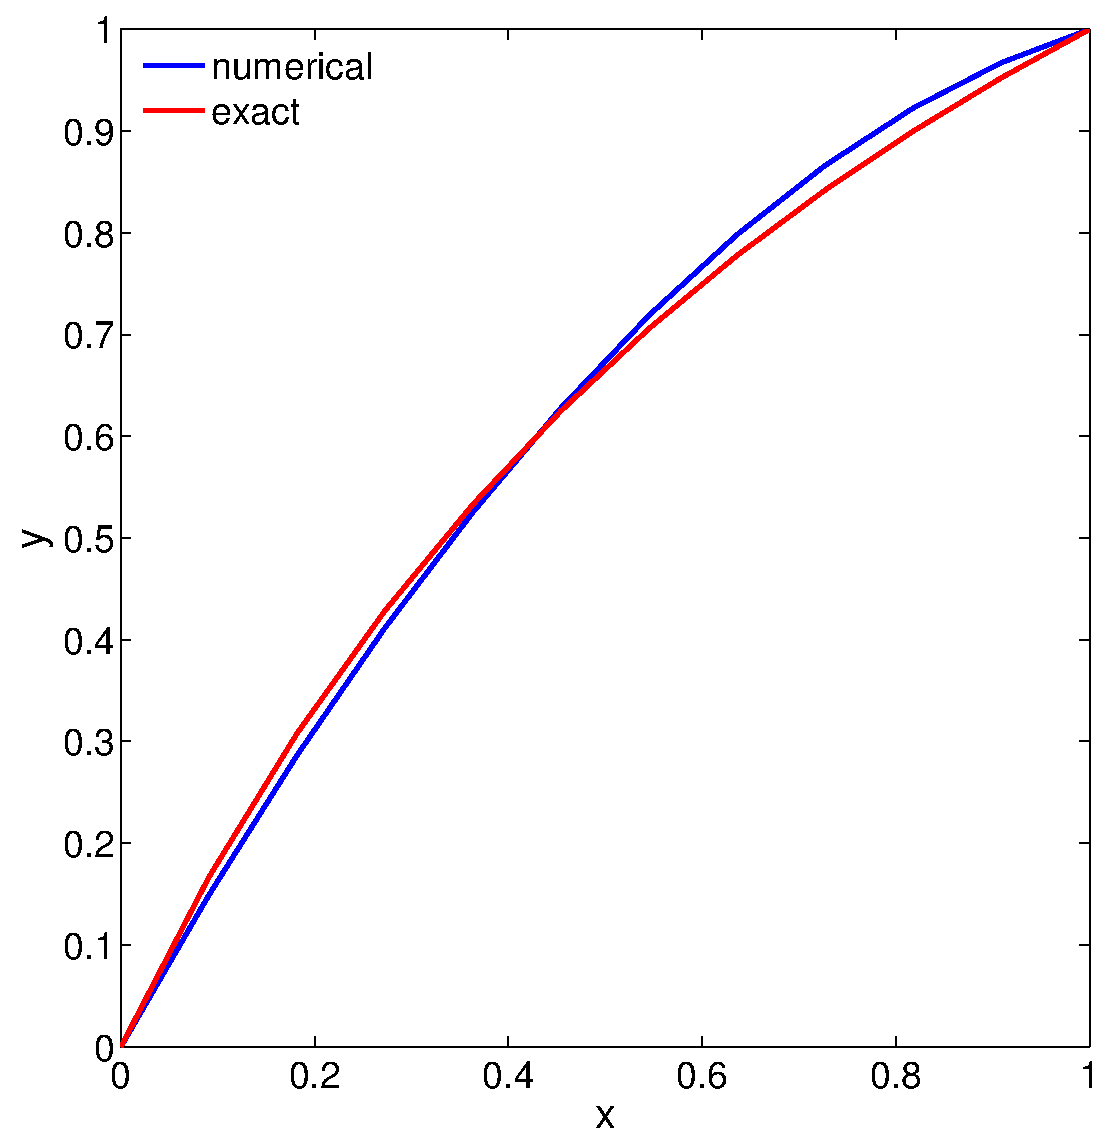
\includegraphics[width=0.45\textwidth]{andy_hw09_prb03_01_m10.pdf}
  \caption{Exact and numerical solutions of the BVP using the Galerkin method with $M=10$.}
\end{figure}

\begin{figure}[h!]
  \centering
    \includegraphics[width=0.45\textwidth]{andy_hw09_prb03_01_m10_error.pdf}
  \caption{Error of the solution to the BVP using the Galerkin method with $M=10$.}
\end{figure}

\begin{figure}[h!]
  \centering
    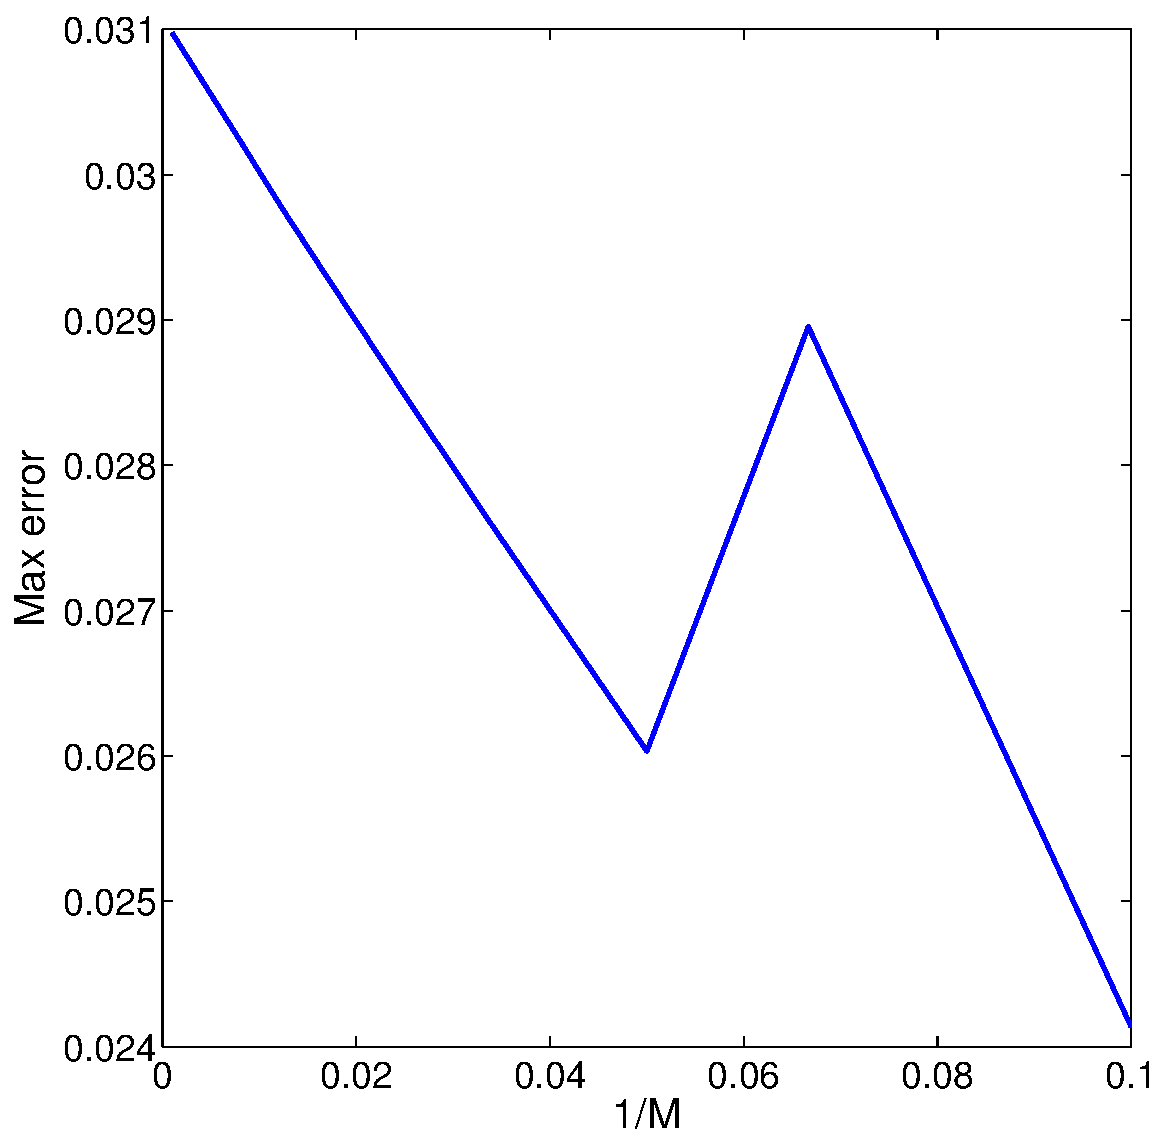
\includegraphics[width=0.45\textwidth]{andy_hw09_prb03_02.pdf}
  \caption{Scaling of the maximum error the Galerkin solution with $(1/M)$.
    All errors are close in magnitude, and do not decrease with $M$ as would be expected. This is likely a coding error on my behalf.}
\end{figure}

\end{enumerate}

\end{document}



